\documentclass[12pt]{beamer}
\usepackage[utf8]{inputenc}
\usepackage[T1]{fontenc}
\usepackage{listings}
\usepackage{tabu}
\beamertemplatenavigationsymbolsempty
\AtBeginSection[]
{
    \begin{frame}
    \frametitle{Table of Contents}
    \tableofcontents[currentsection]
    \end{frame}
}
\lstset{language=C++, basicstyle=\footnotesize, frame=single}

\title{Eulerian path}
\subtitle{Eulerian cycle/path, Chinese postman problem}
\author{beCP Training}
\institute{
\includegraphics[height=12em]{../share/beoi-logo}}

\begin{document}

\frame{\titlepage}

\section{Eulerian cycles and paths}

\begin{frame}
\frametitle{Euler's problem}
Can we make a cycle/path that visits every edge exactly once?
\begin{center}
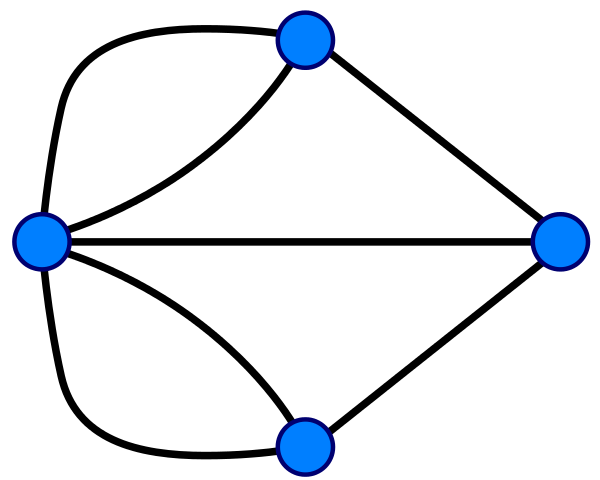
\includegraphics[width=0.6\textwidth]{img/konigsberg}
\end{center}
\end{frame}

\begin{frame}
\frametitle{Eulerian graph}
A eulerian graph is a graph that has a Eulerian cycle (must come back to the start).
\begin{center}
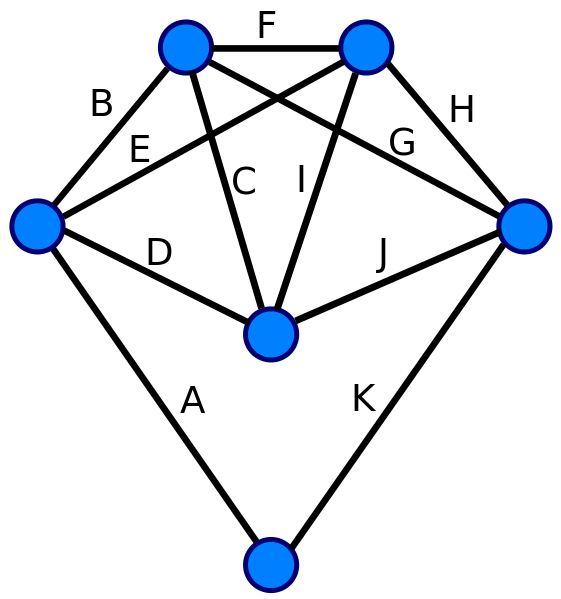
\includegraphics[width=0.5\textwidth]{img/euler-graph}
\end{center}
\end{frame}

\begin{frame}
\frametitle{Semi-eulerian graph}
A semi-eulerian graph is a graph that has a Eulerian cycle \emph{or} path (start and end may differ).
\begin{center}
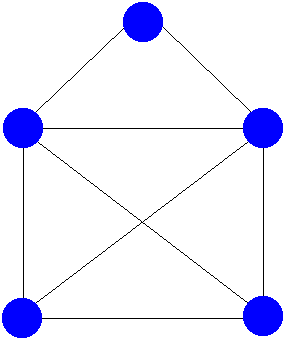
\includegraphics[width=0.4\textwidth]{img/semi-eulerian}
\end{center}
\end{frame}

\begin{frame}
\frametitle{How do we get a Eulerian path/cycle?}
\begin{itemize}
\item The graph must be connected\footnote{The nodes with at least one edge must be connected}
\item For each node except the start and end, we use two edges: one for entering and one for leaving!
\item So all degrees have to be even, except for at most two
\item Actually, those conditions are enough!
\end{itemize}
\begin{center}
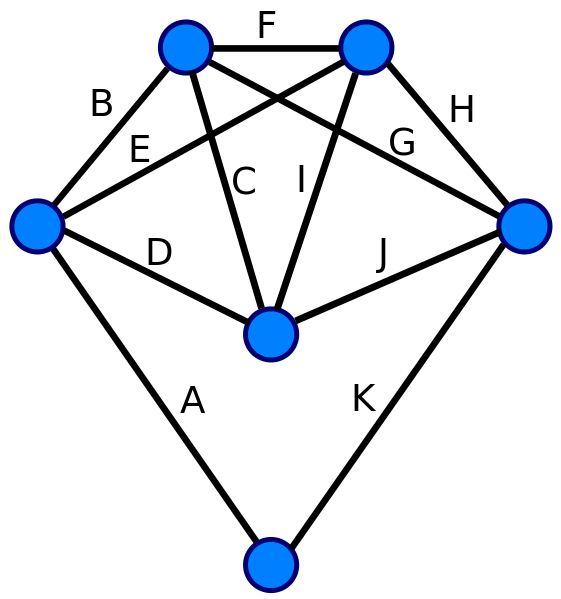
\includegraphics[width=0.25\textwidth]{img/euler-graph}
\qquad
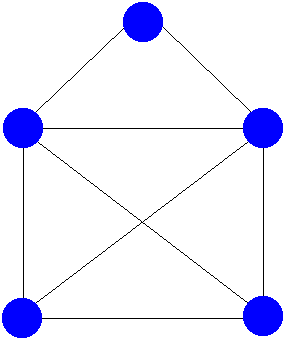
\includegraphics[width=0.22\textwidth]{img/semi-eulerian}
\qquad
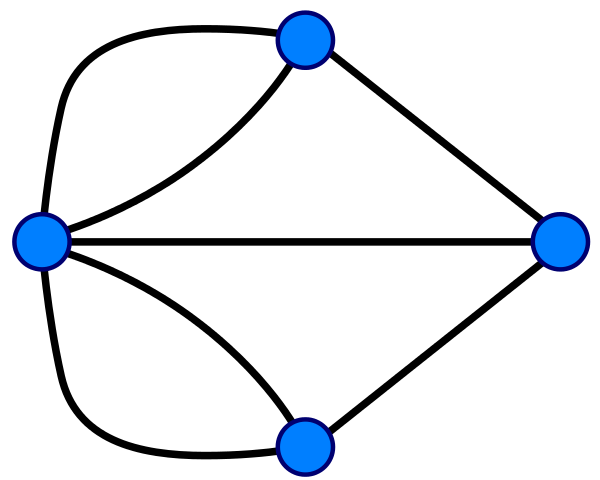
\includegraphics[width=0.3\textwidth]{img/konigsberg}
\end{center}
\end{frame}

\begin{frame}
\frametitle{Criteria for undirected graphs}
\begin{itemize}
\item Eulerian cycle:
    \begin{itemize}
    \item The nodes with at least one edge are in the same connected component
    \item Every node has even degree
    \end{itemize}
\item Eulerian path:
    \begin{itemize}
    \item The nodes with at least one edge are in the same connected component
    \item At most two nodes have odd degree
    \end{itemize}
\end{itemize}
\end{frame}

\begin{frame}
\frametitle{Criteria for directed graphs}
\begin{itemize}
\item Eulerian cycle:
    \begin{itemize}
    \item The nodes with at least one edge are in the same strongly connected component
    \item Every node has equal in-degree and out-degree
    \end{itemize}
\item Eulerian path:
    \begin{itemize}
    \item The nodes with at least one edge are in the same connected component when removing the directions
    \item At most two vertices have a difference of 1 between in-degree and out-degree
    \item All other vertices have equal in-degree and out-degree
    \end{itemize}
\end{itemize}
\begin{center}

\includegraphics[width=.35\linewidth]{img/why-so-many}
\end{center}
\end{frame}

\section{Finding the cycle/path}

\begin{frame}
\frametitle{Traversal strategy}
\begin{itemize}
\item Start at one of the odd-degree nodes (if they exist)
\item Take arbitrary edges and remove them on the way
\item The only possible dead-end is the ending node!
\item If there are edges left, restart in the middle
\end{itemize}
\begin{center}
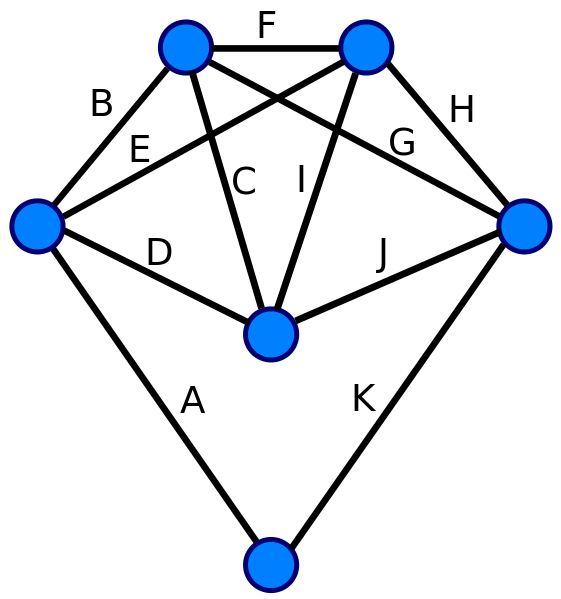
\includegraphics[width=0.4\textwidth]{img/euler-graph}
\end{center}
\end{frame}

\begin{frame}[fragile]
\frametitle{Implementation}
To erase edges, we need to remember an ``edge ID''
\begin{lstlisting}
vector<int> id[MAXV], neigh[MAXV];
bool visited[MAXE]; // which edges have been taken

// Start on an odd-degree node (if possible)
void euler(int u, vector<int> &s)
{
    for (int i=0; i < (int)neigh[u].size(); i++) {
        if (!visited[id[u][i]]) {
            visited[id[u][i]] = true;
            euler(neigh[u][i], s);
        }
    }
    s.push_back(u);
}
\end{lstlisting}
Complexity: $O(V+E)$
\end{frame}

\section{Chinese postman problem}

\begin{frame}
\frametitle{Chinese postman statement}
\begin{itemize}
\item A postman has to make a cycle through every street at least once, while travelling the smallest possible distance.
\item If the graph is Eulerian, then just take a Eulerian cycle
\item Otherwise, there are an even number of odd-degree nodes
\item Let's add edges to make it Eulerian!
\end{itemize}
\begin{center}
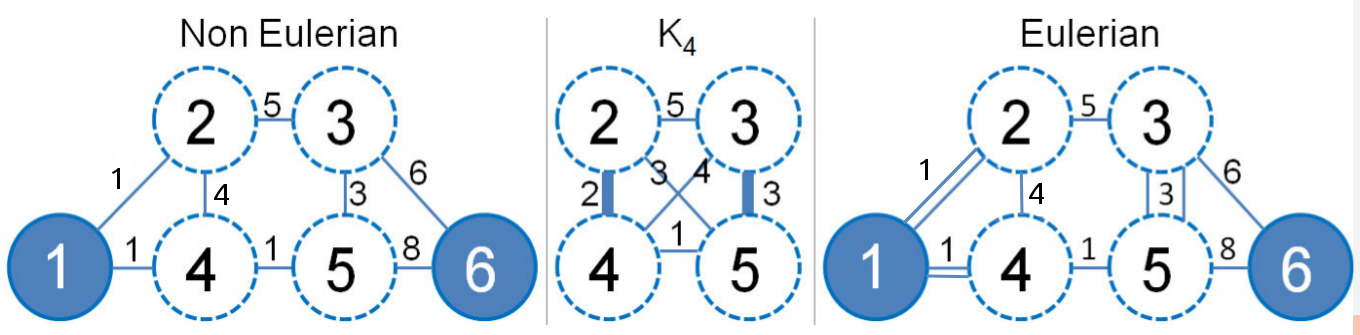
\includegraphics[width=.9\linewidth]{img/cp3-complete}
\end{center}
\end{frame}

\begin{frame}
\frametitle{Choosing the right edges to add}
\begin{itemize}
\item We have to add an edge to every odd-degree node
\item But not change the parity of even-degree node
\item So we have to add paths between pairs of odd-degree nodes
\item Compute the best paths and put it in a graph
\item Find the best pairings with complete search
\end{itemize}
\begin{center}
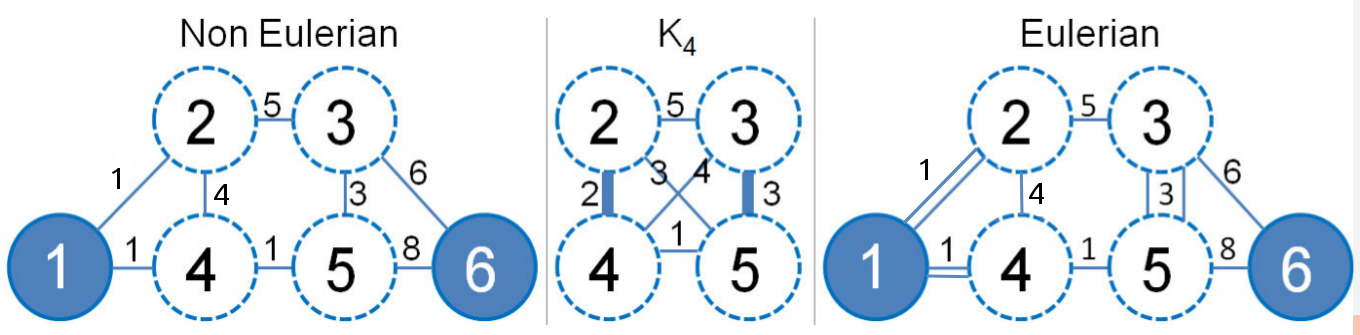
\includegraphics[width=.9\linewidth]{img/cp3-complete}
\end{center}
\end{frame}

\begin{frame}
\frametitle{Sources of figures}
\begin{itemize}
\item \url{https://commons.wikimedia.org/wiki/File:Königsberg_graph.svg}
\item \url{https://commons.wikimedia.org/wiki/File:Labelled_Eulergraph.svg}
\item \url{https://en.wikibooks.org/wiki/File:Eulerian3.png}
\item CP3 book
\end{itemize}
\end{frame}

\end{document}
